\section{System Implementation}

The implementation of the system describes each component as it was implemented in the final system. In this section, the broad functionality of each component is described. Further subsections discuss the overall accuracy and results achieved from the components implemented. \\

\subsection{CoreLoader}

The main Coreloader screen contains all functionality associated with the system. There are options present for selecting particular Kinect feeds, calibrating the Kinect's position and viewing the debug console. Recent patients are also displayed persistently for quick access to the scans and results of previous scans on a particular patient. Configuration options are also possible through Coreloader such as setting the working directory for PARSE files and attributing .PARSE and .PCD scan files to patients. Exporting scans to .PCD is also here so that scans produced by the System can be visualised using the Point Cloud Library toolkit\footnote{Point Cloud Library, http://www.pointclouds.org}. \\

\begin{center}
    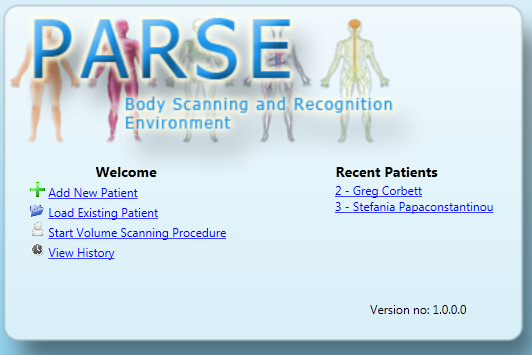
\includegraphics[scale=0.5]{zscreenshots/corewelcome.png}\\
    \caption{CoreLoader welcome screen with toolkit options}
\end{center} \\

\begin{center}
    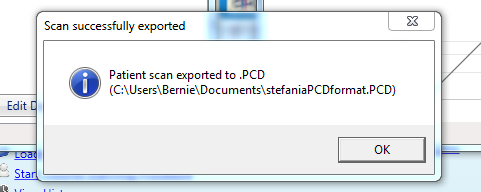
\includegraphics[scale=0.6]{zscreenshots/savetopcd.PNG}\\
    \caption{Confirmation of point cloud file exported to .PCD}
\end{center} \\

\begin{center}
    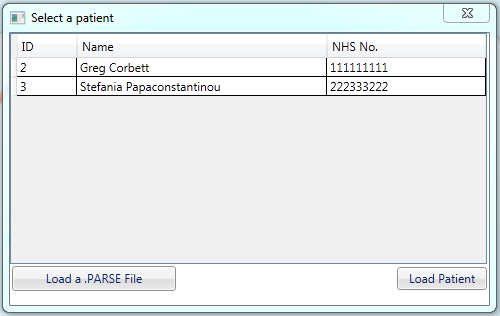
\includegraphics[scale=0.55]{zscreenshots/metaloader.PNG}\\
    \caption{List of patients in the database with associated point cloud or scan information}
\end{center} \\

\begin{center}
    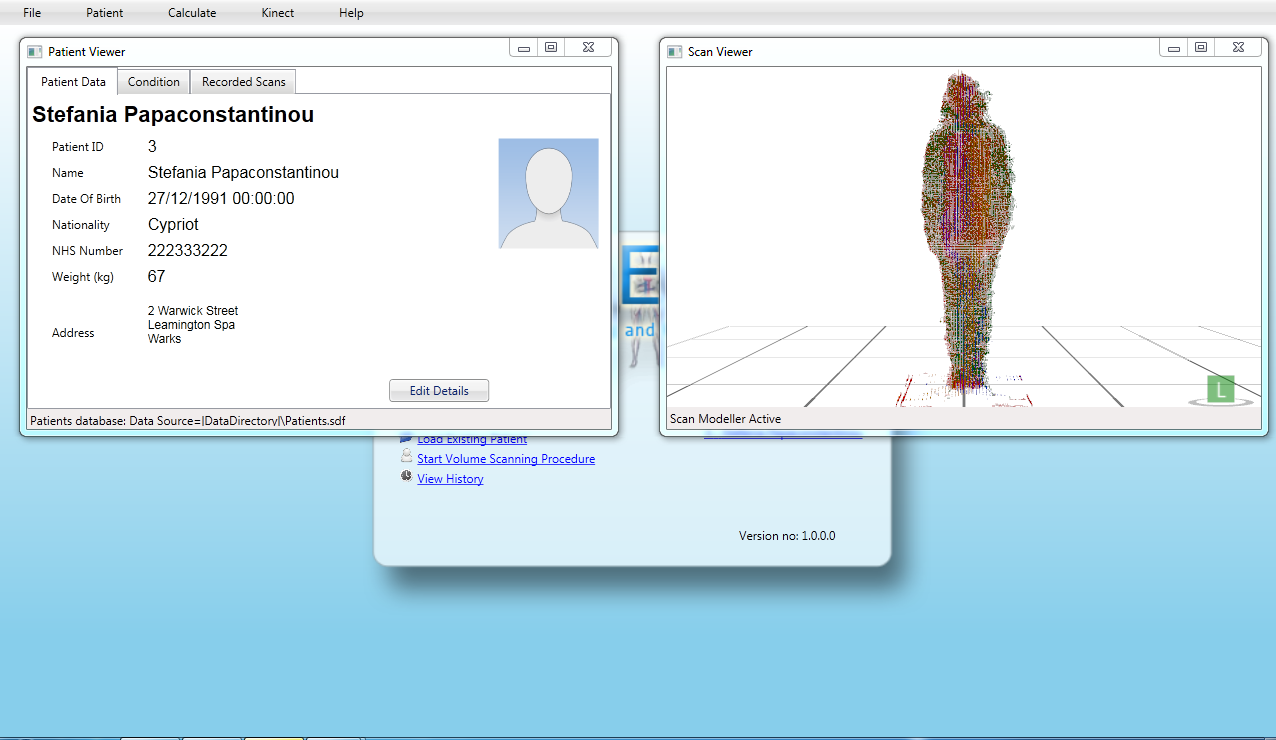
\includegraphics[scale=0.3]{zscreenshots/coreloaderstef.PNG}\\
    \caption{System with scan and associated patient detail displayed}
\end{center} \\


\subsection{ViewLoader}

\begin{center}
    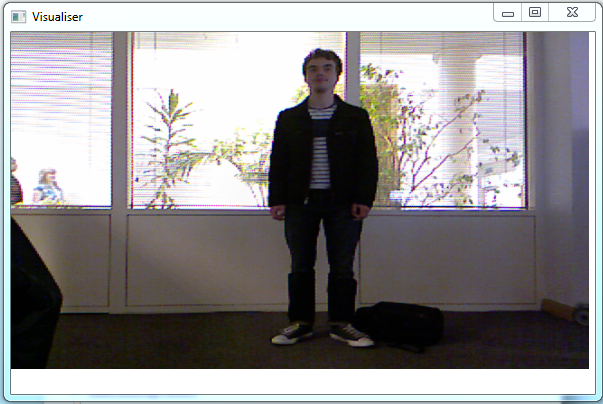
\includegraphics[scale=0.5]{zscreenshots/rgbvisualiser.PNG} \\
    \caption{ViewLoader: Showing the raw RGB feed}
\end{center} \\

Viewloader is capable of displaying raw streams from the Kinect or composite streams that combine multiple views such as depth isolation, colour isolation, or the overlay of a skeleton onto existing feeds. The above image shows the conventional RGB feed from the Kinect. \\

\subsection{ScanLoader}

\begin{center}
    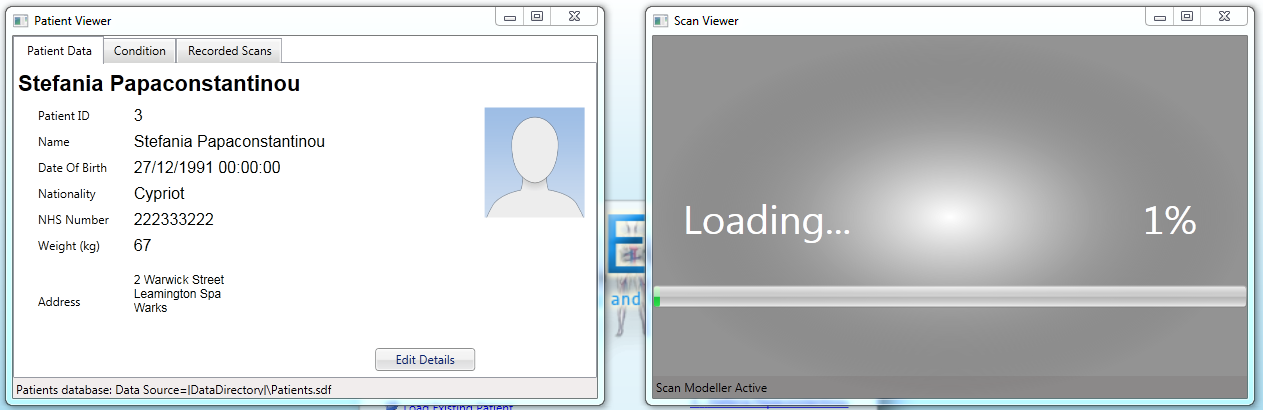
\includegraphics[scale=0.3]{zscreenshots/patientloading.png} \\
    \caption{ScanLoader: The patient data portal (left) and the model viewer loading (right)}
\end{center} \\

\begin{center}
    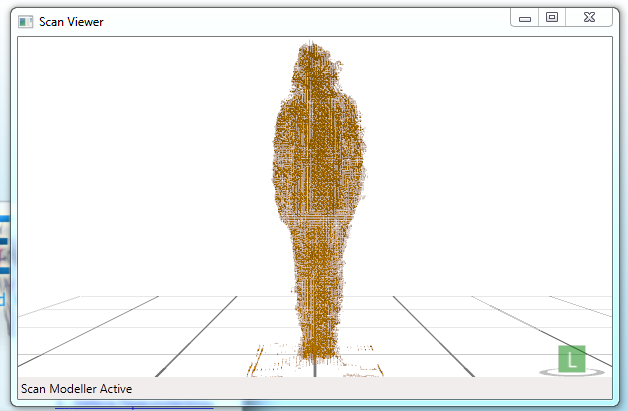
\includegraphics[scale=0.5]{zscreenshots/scanframework.png} \\
    \caption{ScanLoader: 3D model viewport}
\end{center} \\

ScanLoader visualises the registered point clouds from the scan process and allows the model to be viewed from a number of different perspectives and zoom levels. The point cloud visualisation process is resource intensive as approximately 200,000 points are drawn in 3D space. As a result of this, a persistent loading dialog is displayed when the point cloud is being loaded into scan loader or when refining operations are applied to the point cloud. \\

\subsection{HistoryLoader}

\begin{center}
    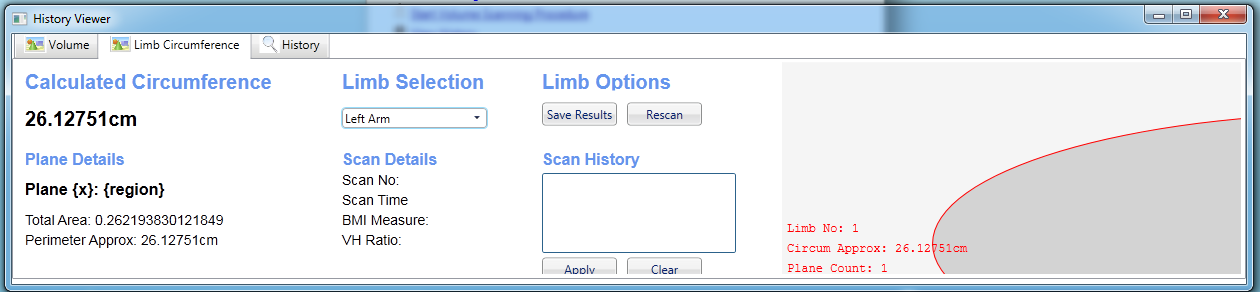
\includegraphics[scale=0.4]{zscreenshots/circumdetail.png}
    \caption{HistoryLoader: Circumference history}
\end{center} \\

\begin{center}
    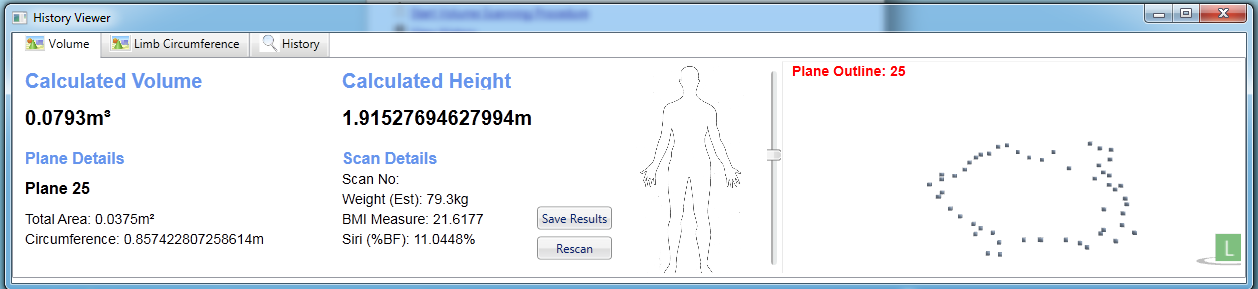
\includegraphics[scale=0.4]{zscreenshots/voldetail.png}
    \caption{HistoryLoader: Volume, height \& plane history}
\end{center} \\

\begin{center}
    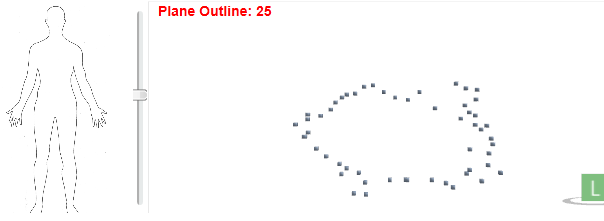
\includegraphics[scale=0.75]{zscreenshots/volumevisualisation.png}
    \caption{HistoryLoader: Plane viewer}
\end{center} \\

The HistoryLoader component of the system visualises the volume and circumference calculation results along with visualisations related to the extrcted planes from the point cloud as well as the visualisation for the approximation of the circumference of the limbs. In each component, different metrics can be visualised for volume in terms of the different planes of the body as well as the circumference for each limb that has been partitioned. These results can then be saved or refined during a rescan procedure. \\

\subsection{PatientLoader}

\begin{center}
    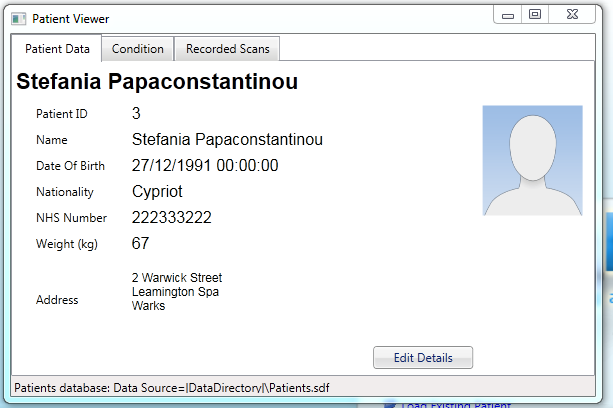
\includegraphics[scale=0.5]{zscreenshots/patientdetail.png} \\
    \caption{PatientLoader: Patient information pane}
\end{center} \\

The PatientLoader presents the patient detail recovered from the database when a patient's scans for either volume/limb circumference or markerless recognition purposes is loaded. PatientLoader also provides the ability to apply new markerless measurements and recover old measurements. Patient information such as personal details and patient conditions can also be added here. \\

\subsection{MeasurementLoader}
MeasurementLoader presents the mechanism for adding a new body-relative scan position with a hand-held sensor. Clear instructions are displayed, indicating to the users how to progress.\\

\begin{enumerate}
    \item Wait for two people to be in view
    \item Search for the sensor device
    \item Use the sensor's location, in combination with the skeletal data, to identify the doctor and the patient
    \item When the sensor is held still for 10 seconds, the system automatically runs the capture routine.
\end{enumerate} \\

\begin{center}
    \setlength\fboxsep{0pt}
    \setlength\fboxrule{0.5pt}
    \fbox{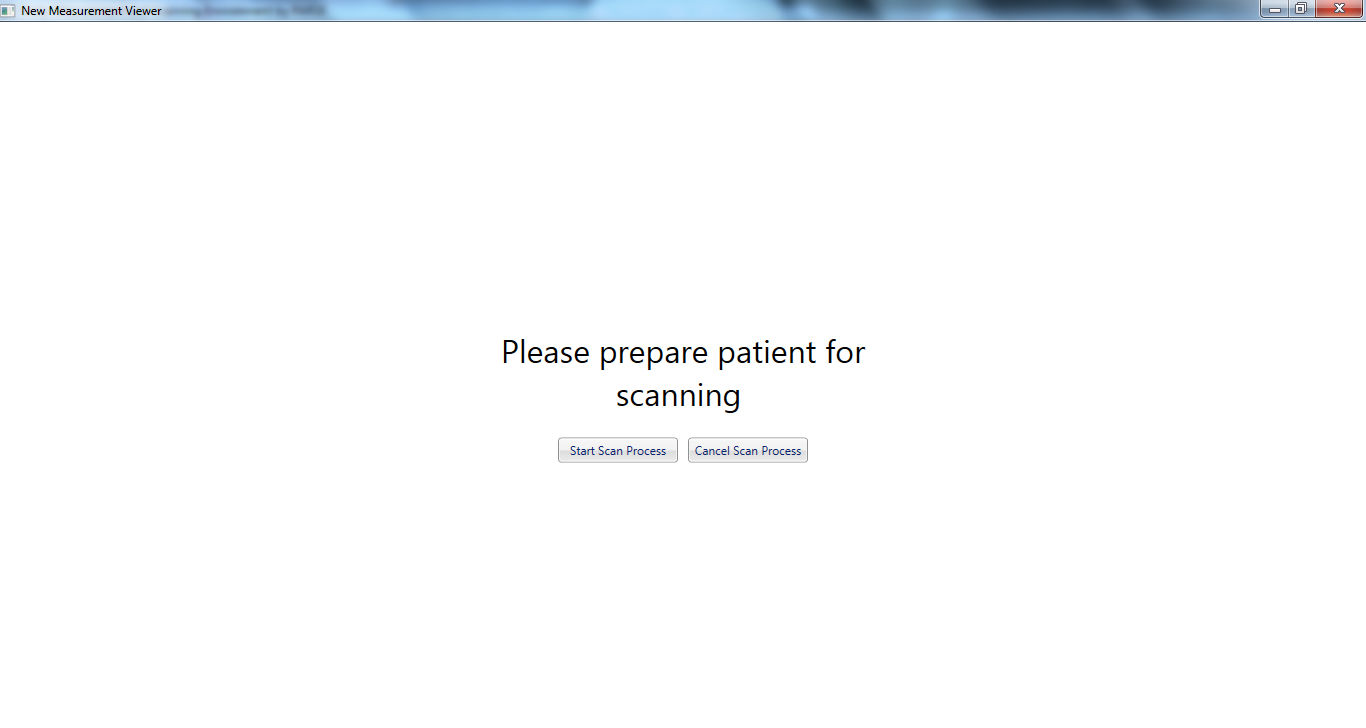
\includegraphics[scale=0.25]{zscreenshots/MeasurementLoader.png}}\\
    \caption{MeasurementLoader: Ready to start a scan}
\end{center} \\

\begin{center}
    \setlength\fboxsep{0pt}
    \setlength\fboxrule{0.5pt}
    \fbox{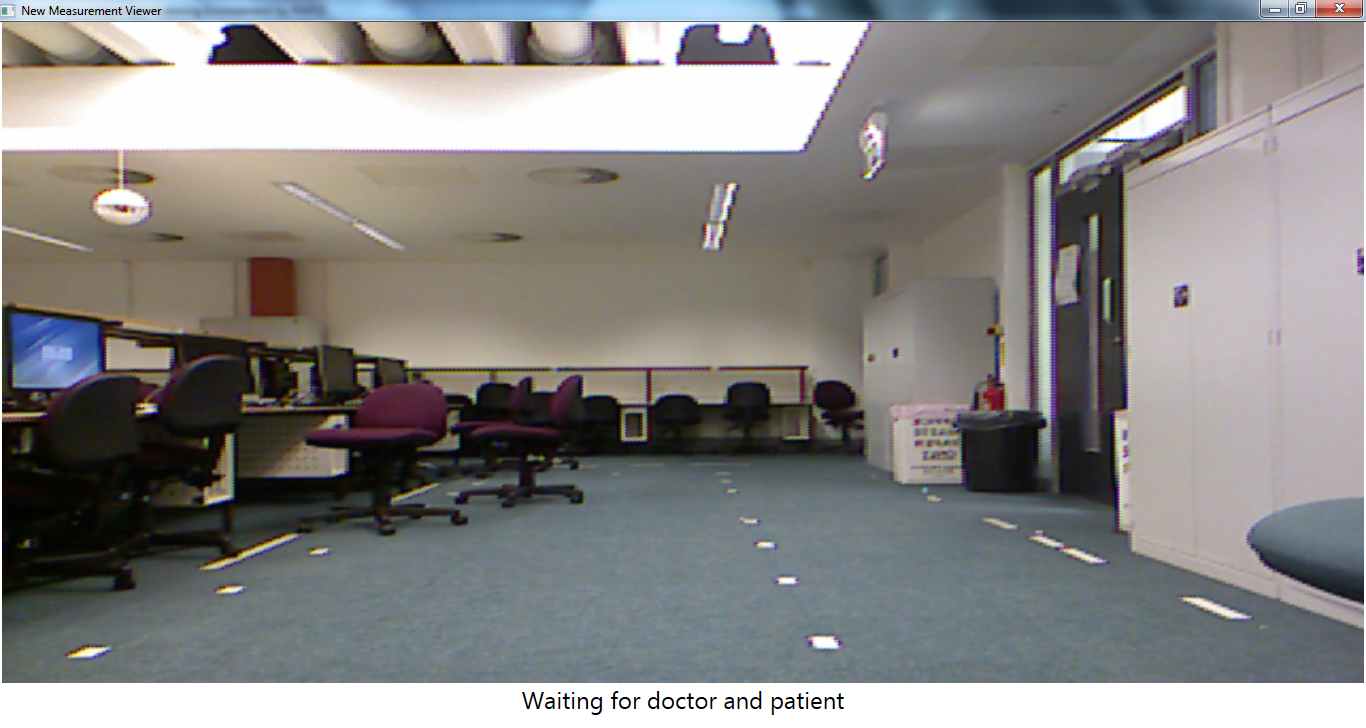
\includegraphics[scale=0.25]{zscreenshots/MeasurementLoader2.png}}\\
    \caption{MeasurementLoader: The large, clear display indicates the next step}
\end{center}
